\subsection{UCW1 - Preparazione ambiente}
\label{sub:ucw1}

%TODO: Add correct image
% Se uno use case esce dalla post allora non mettiamo in scenario secondario ma in estensione
% se invece la post rimane la stessa non è estensione.

\begin{figure}[h]
    \centering
    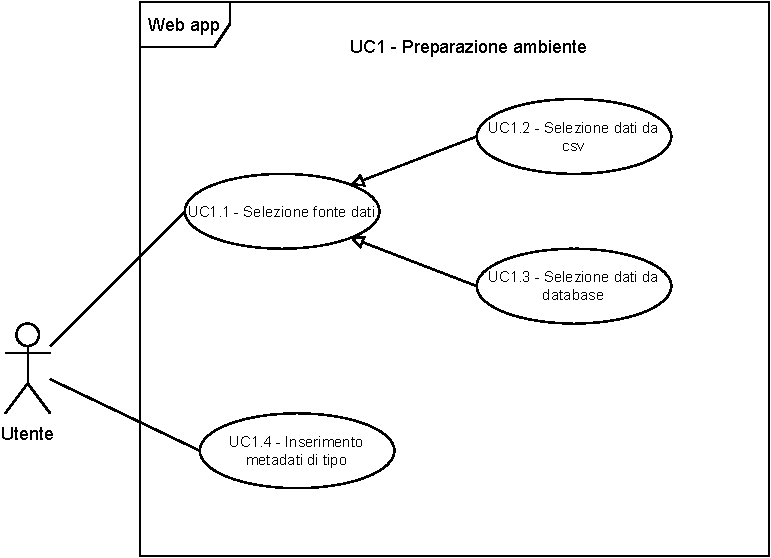
\includegraphics[width=0.7\textwidth]{diagrammi/UC1.pdf}
    \caption{Diagramma rappresentante UCW1}
    \label{fig:UCW1}
\end{figure}


\begin{itemize}
    \item \textbf{Descrizione}: L'utente prepara l'applicativo HD Viz alla visualizzazione dei dati selezionando la fonte del suo dataset.
	
    \item \textbf{Attore primario}: Utente;
        
    \item \textbf{Precondizione}:   L'applicazione è in esecuzione;

    \item \textbf{Postcondizione}:  Viene selezionata la fonte dei dati desiderata;

	\item \textbf{Scenario principale}:
		\begin{enumerate}
			\item L'utente seleziona l'opzione di aggiunta dei dati;
            \item L'utente seleziona la fonte dei dati da importare;
        \end{enumerate}
   
\end{itemize}

\subsubsection{UCW1.1 - Selezione fonte}
\label{ssub:ucw1.1}
\begin{itemize}
    \item \textbf{Descrizione}: L'utente decide di impostare l'ambiente scegliendo la fonte di un dataset;

    \item \textbf{Attore primario}: Utente;
        
    \item \textbf{Precondizione}:   L'applicazione è in esecuzione;

    \item \textbf{Postcondizione}:  Viene selezionata la fonte del dataset;

	\item \textbf{Scenario principale}:
		\begin{enumerate}
			\item L'utente seleziona l'opzione di aggiunta dei dati:
        \end{enumerate}

        \item \textbf{Generalizzazioni}:
        \begin{enumerate}
            \item Selezione dell'opzione file csv (\hyperref[ssub:ucw1.2]{UCW1.2});
            \item Selezione dell'opzione database (\hyperref[ssub:ucw1.3]{UCW1.3}).
        \end{enumerate}
\end{itemize}


\subsubsection{UCW1.2 - Selezione del file csv}
\label{ssub:ucw1.2}
\begin{itemize}
    \item \textbf{Descrizione}: L'utente seleziona un file csv del suo dispositivo;

    \item \textbf{Attore primario}: Utente;
    
    \item \textbf{Precondizione}:   L'applicazione è in esecuzione;
    \item \textbf{Postcondizione}:  Viene selezionato un file csv;

	\item \textbf{Scenario principale}:
		\begin{enumerate}
			\item L'utente seleziona l'opzione di aggiunta dei dati mediante file;
			\item L'utente seleziona il file csv di dati da importare.
        \end{enumerate}
\end{itemize}

\subsubsection{UCW1.3 - Selezione del database}
\label{ssub:ucw1.3}
\begin{itemize}
    \item \textbf{Descrizione}: L'utente seleziona l'input da database e un file di configurazione;
	
    \item \textbf{Attore primario}: Utente;
    
    \item \textbf{Precondizione}:   L'utente decide di caricare i dati mediante un database;
    \item \textbf{Postcondizione}:  Viene selezionato l'input da database e la configurazione desiderata;

	\item \textbf{Scenario principale}:
		\begin{enumerate}
			\item L'utente seleziona l'input da database;
			\item L'utente seleziona una delle impostazioni di configurazione predefiniti.
        \end{enumerate}

\end{itemize}
